\documentclass[pdftex,a4paper,11pt]{article} 
%\documentclass[pdftex,a4paper,11pt]{report} 
%\usepackage[utf8]{inputenc}
%\usepackage[frenchb]{babel}
\usepackage[pdftex]{graphicx}
\usepackage{amsmath}
\usepackage{amssymb}
\usepackage{subfigure}
\usepackage{hyperref}
\usepackage{listings}
\usepackage{color}

\lstset{language=python,numbers=left,breaklines=true}

\hypersetup{
	pdftoolbar=true,                    % show Acrobat’s toolbar ?
	pdfmenubar=true,                    % show Acrobat’s menu ?
	pdffitwindow=true,                  % page fit to window when opened
	pdftitle={Arm model},                    % title
	pdfauthor={Olivier Sigaud},         % author
	pdfsubject={Arm model},                  % subject of the document
	pdfnewwindow=true,                  % links in new window
	pdfkeywords={Arm model},                 % list of keywords
	colorlinks=true,                    % false: boxed links; true: colored links
	linkcolor=black,                    % color of internal links
	citecolor=black,                    % color of links to bibliography
	filecolor=black,                    % color of file links
	urlcolor=black                      % color of external links
}

%\newcommand{\reels}{\mathbb{R}}

\begin{document}

\title{A motor control model}
\author{Thomas Beucher}
\maketitle

\section*{Abstract}
Two basic phenomena interact in the way the speed of our reaching movements is determined.
First, we tend to reach faster a target that looks more rewarding, despite the additional muscular cost
of a faster movement.
Second, when we need to be more precise, our movement takes more time.
So far, these two phenomena have been studied in isolation despite their obvious interdependency.
In particular, two recent computational models of motor control address the first phenomenon. They explain the emergence of the time of movement as resulting from a cost-benefit trade-off arising from the summation of a temporally discounted reward and a cost that increases for faster movements.
However, these models do not account for the second phenomenon, i.e. the dependency between movement time and precision requirements, resulting in a speed-accuracy trade-off and formally expressed by Fitts' law. Another model addresses the role of this speed-accuracy trade-off in determining movement time, but does not take the cost of movement into account.

In this paper, we propose a framework that unifies the cost-benefit trade-off and the speed-accuracy trade-off to explain movement properties related to time.
With respect to the cost-benefit trade-off models, precision constraints are incorporated through the derivation of a new optimization criterion that considers probabilistic reaching of a rewarding target that may be missed if the motion is too fast.

Using this computational model, we investigate the more global trade-off arising from the interactions between movement time, cost and accuracy. We show that this model accounts for Fitts' law and for other well-established results in the motor control literature.


\section{Arm model}

The plant is a two degrees-of-freedom (dofs) planar arm controlled by 6 muscles, illustrated in Fig.~\ref{fig:arm_model}.
There are several such models in the literature. The model described in \cite{Kambara2009} lies in the vertical
plane so it takes the gravity force into account. Most other models are defined in the saggital plane and
ignore gravity effects. They all combine a simple two dofs planar rigid-body dynamics model with a 
muscular actuation model. The differences between models mostly lie in the latter component.

\begin{figure*}[hbt]
\centering
	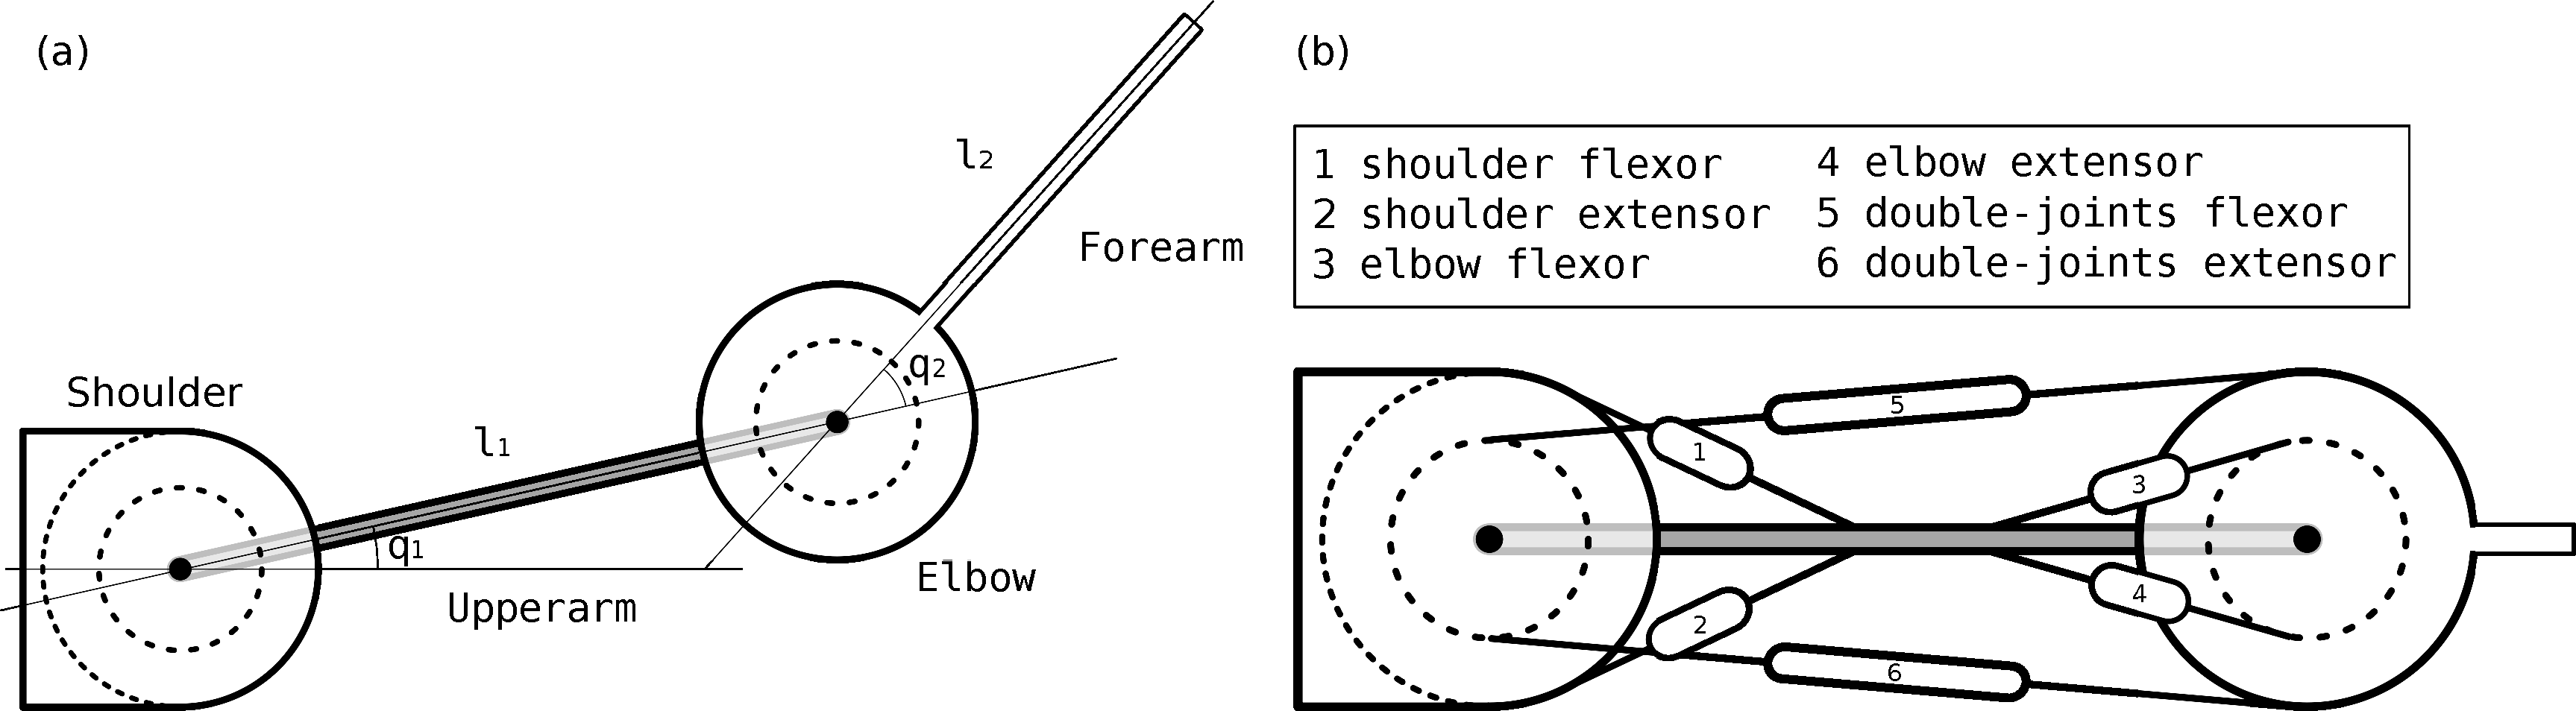
\includegraphics[width=0.9\columnwidth]{figures/arm_model_horiz.pdf}
	\caption{Arm model. (a) Schematic view of the arm mechanics. (b) Schematic view of the muscular actuation of the arm, where each number represents a muscle whose name is in the box.}
	\label{fig:arm_model}
\end{figure*}

Table~\ref{arm_model_params} in Appendix~\ref{sec:params} reminds the nomenclature of all the parameters and variables of the arm model. 

\subsection{Arm parameters}
\label{sec:arm_parameters}
All parameters of the arm are defined in the file \textit{setupArmParameters} and implemented in the class \textit{ArmParameters}.
This class defines the following functions:
\begin{itemize}
\item[\textit{readSetupFile}]: Reads the setup file.
\item[\textit{massMatrix}]: Defines the inertia matrix parameters.
\item[\textit{BMatrix}]: Defines the damping matrix \textbf{B}, with
$\textbf{B} = \begin{bmatrix}
           .05 & .025 \\
          .025 & .05
     \end{bmatrix} \dot{q}.$\\
\item[\textit{AMatrix}]: Defines the moment arm matrix A.
\begin{align*}
  \textbf{A}^\top        & = \begin{bmatrix}
    a_{1} & a_{2} & a_{3} & a_{4} & a_{5} & a_{6} \\
    a_{7} & a_{8} & a_{9} & a_{10} & a_{11} & a_{12} \\
  \end{bmatrix} \\
  & = \begin{bmatrix}
    .04 & -.04 &    0 &     0 & .028 & -.035 \\
    0 &    0 & .025 & -.025 & .028 & -0.35 \\
  \end{bmatrix}\\
\end{align*}
\end{itemize}
All the arm parameters values are summarized in \hyperref[ArmParamTable]{Table~\ref{ArmParamTable}} in Appendix~\ref{sec:params}.

\subsection{Muscles parameters}
\label{sec:muscle_parameters}
All muscles parameters are defined in the file \textit{setupMusclesParameters} and implemented in the class \textit{MusclesParameters}.
This class defines the following functions:
\begin{itemize}
\item[\textit{fmaxMatrix}]: Defines the matrix of the maximum force exerted by each muscle.
\begin{align*}
\textbf{f}_\textbf{max}   & = \begin{pmatrix}
f_{\max1} &0&0&0&0&0\\
0& f_{\max2}&0&0&0&0\\
0&0& f_{\max3} &0&0\\
0&0&0& f_{\max4} &0&0\\
0&0&0&0& f_{\max5} &0\\
0&0&0&0&0& f_{\max6}\\
\end{pmatrix} \\& = \begin{pmatrix}
700 &0&0&0&0&0\\
 0&382&0&0&0&0\\
0&0 & 572 & 0&0&0\\
0&0&0&445 &0&0\\
0&0&0&0&159 &0\\
0&0&0&0&0&318
\end{pmatrix}\\
\end{align*}
\item[\textit{activationVectorInit}]: Initializes the muscular activation vector. (Create the vector initializes to zero)
\item[\textit{activationVectorUse}]: Builds the muscular activation vector given its 6 components.
\end{itemize}
All the muscles parameters values are summarized in \hyperref[MuscleParamTable]{Table 3} in Appendix~\ref{sec:params}.

\subsection{Rigid-body dynamics}
\label{sec:arm_dynamics}
The rigid-body dynamics equation of a mechanical system is:

 \begin{equation}
\label{eq:rbd}
    \ddot{q} = \textbf{M}(q)^{-1} (\tau - \textbf{C}(q, \dot{q}) - \textbf{g}(q)  - \textbf{B} \dot{q}) 
\end{equation}

where $\textbf{q}$ is the current articular position, $\dot{q}$ the current articular speed, $\ddot{q}$ the current articular acceleration, $\textbf{M}$ the inertia matrix, $\textbf{C}$ the Coriolis force vector, $\boldsymbol{\tau}$ the segments torque, $\textbf{g}$ the gravity force vector and $\textbf{B}$ a damping term that contains all unmodelled effects.
Here, $\textbf{g}$ is ignored since the arm is working in the sagittal plane.
All angles are expressed in radians.
We can compute the inertia matrix as:
$
\textbf{M} = \begin{bmatrix}
           k_1 + 2 k_2 \cos(q_2)   &  k_3 + k_2 \cos(q_2) \\%[0.3em]
           k_3 + k_2 \cos(q_2)     &  k_3
          \end{bmatrix}
$, with $k_1 = d_1 + d_2 + m_2 l_1^2, ~ k_2 = m_2 l_1 s_2, ~ k_3 = d_2$ where $d_i$, $m_i$, $l_i$ and $s_i$ are parameters of the arm previously defined in Section~\ref{sec:arm_parameters}.

The Coriolis force vector is given by
$$
\textbf{C} = \begin{bmatrix}
           - \dot{q_2} (2 \dot{q_1} + \dot{q_2}) k_2 \sin(q_2)\\
            \dot{q_1}^2 k_2 \sin(q_2)
          \end{bmatrix}.
$$

The computation of the torque $\tau$ exerted on the system given an input muscular actuation $\textbf{u}$ is explained in the section~\ref{sec:muscular_actuation}.

Equation~\ref{eq:rbd} is implemented in the class \textit{ArmDynamics} line 57:
{\bf renumber the lines}
\begin{lstlisting}
ddotq = np.dot(Minv,(Gamma - C - np.dot(armP.B, dotq)))
\end{lstlisting}
where \textit{np} refere to the numpy library in python.
We also find in this class all elements of Equation~\ref{eq:rbd}:
\begin{lstlisting}
#Inertia matrix
M = np.array([[armP.k1+2*armP.k2*math.cos(q[1,0]),armP.k3+armP.k2*math.cos(q[1,0])],[armP.k3+armP.k2*math.cos(q[1,0]),armP.k3]])
#Coriolis force vector
C = np.array([[-dotq[1,0]*(2*dotq[0,0]+dotq[1,0])*armP.k2*math.sin(q[1,0])],[(dotq[0,0]**2)*armP.k2*math.sin(q[1,0])]])
#inversion of M
Minv = np.linalg.inv(M)
#torque term
Q = np.diag([q[0,0], q[0,0], q[1,0], q[1,0], q[0,0], q[0,0]])
#the segment torque
Gamma = np.dot((np.dot(armP.At, musclesP.fmax)-np.dot(musclesP.Knulle, Q)), U)
\end{lstlisting}

\subsection{Muscular actuation}
\label{sec:muscular_actuation}
Our muscular actuation model is taken from \cite{katayama93} (pp.~356-357) through \cite{mitrovic08_SAB}.
It is a simplified version of the one described in \cite{li2006} in the sense that it uses
a constant moment arm matrix $\textbf{A}$ whereas \cite{li2006} is computing this matrix as
a function of the state of the arm.

Finally, given an action $\textbf{u}$ corresponding to a raw muscular activation as output of the
controller, the muscular activation
is augmented with Gaussian noise using $\textbf{\~{u}} = \log(\exp(\kappa \times \textbf{u}_t \times (1+\mathcal{N}(0,\textbf{I}\sigma_u^2))) + 1) / \kappa$, where $\times$ refers to the element-wise multiplication, $\textbf{I}$ is a $6 \times 6$ identity matrix.
and $\kappa = 25$ is the Heaviside filter parameter, and the input torque 
is computed as $\boldsymbol{\tau} = \textbf{A}^\top ( \textbf{f}_\textbf{max} \times \textbf{\~{u}} )$.

\appendix
\section{Nomenclature of arm parameters}
\label{sec:params}

\begin{table}[hbt]
\caption{Parameters of the arm model.}
\begin{center}
\begin{tabular}{|c|c|}
\hline  
$m_i$ & mass of segment $i$ ($kg$) \\
$l_i$ & length of segment $i$ ($m$) \\
$s_i$ & inertia of segment $i$ ($kg.m^2$) \\
$d_i$ & distance from the center of \\
      &  segment $i$ to its center of mass ($m$) \\
$\kappa$ & Heaviside filter parameter \\
$\textbf{A}$ & moment arm matrix ($\in \mathbb{R}^{6 \times 2}$)\\
$\textbf{f}_{\textbf{max}}$ & maximum muscular tension ($\in \mathbb{R}^6$)\\
$\textbf{M}$ & inertia matrix ($\in \mathbb{R}^{2 \times 2}$)\\
%$\mat{J}$ & Jacobian matrix \\
$\textbf{C}$ & Coriolis force ($N.m \in \mathbb{R}^2$)\\
$\tau$ & segments torque ($N.m \in \mathbb{R}^2$)\\

$\textbf{B}$ & damping term ($N.m \in \mathbb{R}^2$)\\
$\textbf{u}$ & raw muscular activation (action) ($\in [0,1]^6$)\\
$\sigma_u^2$ & multiplicative muscular noise ($\in [0,1]^6$)\\
$\tilde{u}$ & filtered noisy muscular activation ($\in [0,1]^6$)\\
$\textbf{q}^*$ & target articular position ($rad \in [0,2\pi[^2$)\\
$\textbf{q}$ & current articular position ($rad \in [0,2\pi[^2$)\\
$\dot{q}$ & current articular speed ($rad.s^{-1}$)\\
$\ddot{q}$ & current articular acceleration ($rad.s^{-2}$)\\
\hline
\end{tabular}
\end{center}
\label{arm_model_params}
\end{table}

\begin{table}[hbt]
\caption{Parameters of the arm.}
\begin{center}
\begin{tabular}{|c|c|c|}
\hline  
$\textbf{l}_{\textbf{1}}$ & arm length ($m$) & 0.3\\
$\textbf{l}_{\textbf{2}}$ & forearm length ($m$) & 0.35\\
$\textbf{m}_{\textbf{1}}$ & arm mass ($kg$) & 1.4\\
$\textbf{m}_{\textbf{2}}$ & forearm mass ($kg$) & 1.1\\
$\textbf{s}_{\textbf{1}}$ & arm inertia ($kg.m^2$) & 0.11\\
$\textbf{s}_{\textbf{2}}$ & forearm inertia ($kg.m^2$) & 0.16\\
$\textbf{d}_{\textbf{1}}$ & distance from the center of segment 1 to its center of mass ($m$) & 0.025\\
$\textbf{d}_{\textbf{2}}$ & distance from the center of segment 2 to its center of mass ($m$) & 0.045\\
$\textbf{k}_{\textbf{6}}$ & damping term & 0.05\\
$\textbf{k}_{\textbf{7}}$ & damping term & 0.025\\
$\textbf{k}_{\textbf{8}}$ & damping term & 0.025\\
$\textbf{k}_{\textbf{9}}$ & damping term & 0.05\\
$\textbf{a}_{\textbf{1}}$ & moment arm matrix & 0.04\\
$\textbf{a}_{\textbf{2}}$ & moment arm matrix & -0.04\\
$\textbf{a}_{\textbf{3}}$ & moment arm matrix & 0.0\\
$\textbf{a}_{\textbf{4}}$ & moment arm matrix & 0.0\\
$\textbf{a}_{\textbf{5}}$ & moment arm matrix & 0.028\\
$\textbf{a}_{\textbf{6}}$ & moment arm matrix & -0.035\\
$\textbf{a}_{\textbf{7}}$ & moment arm matrix & 0.0\\
$\textbf{a}_{\textbf{8}}$ & moment arm matrix & 0.0\\
$\textbf{a}_{\textbf{9}}$ & moment arm matrix & 0.025\\
$\textbf{a}_{\textbf{10}}$ & moment arm matrix & -0.025\\
$\textbf{a}_{\textbf{11}}$ & moment arm matrix & 0.028\\
$\textbf{a}_{\textbf{12}}$ & moment arm matrix & -0.035\\
\hline
\end{tabular}
\end{center}
\label{ArmParamTable}
\end{table}

\begin{table}[hbt]
\caption{Parameters of the muscles.}
\begin{center}
\begin{tabular}{|c|c|c|}
\hline  
$\textbf{f}_{\textbf{max1}}$ & Maximum force exerted by the shoulder flexor & 700\\
$\textbf{f}_{\textbf{max2}}$ & Maximum force exerted by the shoulder extensor & 382\\
$\textbf{f}_{\textbf{max3}}$ & Maximum force exerted by the elbow flexor & 572\\
$\textbf{f}_{\textbf{max4}}$ & Maximum force exerted by the elbow extensor & 445\\
$\textbf{f}_{\textbf{max5}}$ & Maximum force exerted by the double-joints flexor & 159\\
$\textbf{f}_{\textbf{max6}}$ & Maximum force exerted by the double-joints extensor & 318\\
\hline
\end{tabular}
\end{center}
\label{MuscleParamTable}
\end{table}

\bibliographystyle{abbrv}
\bibliography{twoDarm}

\end{document}
